\documentclass[11pt]{article}
\usepackage[margin=1in]{geometry}
\usepackage{pdfpages}
\usepackage[sfdefault]{GoSans}
\usepackage{longtable}
\usepackage{array}
\usepackage{verbatim}
\usepackage{graphicx}
\graphicspath{ {./images/} }
\linespread{1,5}


\begin{document}

\includepdf[]{DeckblattPflichtenheft.pdf}
\title{Pflichtenheft}

\author{Die kranken Schwestern}

\tableofcontents
\pagebreak

\section{Zielbestimmung}
\subsection{Musskriterien}
Das Programm soll dazu dienen, Zelluläre Automaten auf einem 2-D orthogonalen Spielfeld darstellen zu können. Dazu werden als Beispiel die Regeln für Conway`s Game of Life verwendet.
Hierzu sind unbedingt die folgenden Features erforderlich:

\par



\begin{longtable}[m]{|m{2.2cm}|m{4cm}|m{8cm}|}
\hline
M0001     & UI & Das Programm muss eine graphische Oberfläche haben.  \\
\hline
M0002 & Scope & •   Es soll ein zellulärer Automat mit möglichst großer Freiheit definiert und simuliert werden können.  \\
\hline
M0003 & Darstellung Spielfeld & •   Die Darstellung des Zellulären Automaten erfolgt über eine 2 Dimensionale Matrix aus Quadraten deren Farbe und Helligkeit den Zustand eines Feldes wiedergeben. \\
\hline
M0004 & Transitionsregeleditor & Die Transitionsregeln sollen über eine definierte und im Handbuch dokumentierte Syntax (invers Polnische Notation, ggf. auch mathematische Schreibweise) formuliert werden können. Der neue Zustand einer Zelle darf dabei von der Zelle selbst, sowie von den umliegenden acht benachbarten Zellen abhängen. Ihr Status wird in Variablen bereitgestellt.\\
\hline
M0005 & Spielfeldaufbau & Das Spielfeld soll als 2-D Array von Integerwerten ausgeführt sein, welche den Zellzustand repräsentieren.\\
\hline
0006 & Spielfeldgröße & Die Spielfeldgröße soll vor Simulationsstart vom Benutzer über (Text-)Eingabefelder festgelegt werden können.\\
\hline
M0007 & Speichern \& Laden & Spielfeldzustand und Transitionsregeln sollen seperat gespeichert und geladen werden können.  \\
\hline
M0008 & Einfügen & Es sollen Figuren in das Spielfeld eingefügt werden können. Dies soll so geschehen, dass Figuren als Spielstände mit kleinerer Feldgröße als ganzes geladen und eingefügt werden können. \\
\hline
M0009 & Navigation & es soll möglich sein, das Spielfeld mit Zoom und Pan verschieden zu betrachten. \\
\hline
M0010 & Spielfeldmanipulation & Der Zustand einer Zelle soll durch Mausklick darauf auf einen wählbaren Wert einstellbar sein. Das Wählen des Werts soll durch ein Texteingabefeld auf der Benutzeroberfläche erfolgen. Details in der Beschreibung der Benutzeroberfläche.\\
\hline
M0011 & Topologie & Das Randverhalten des Spielfelds soll zwischen begrenztem Rechteck und Torus (Zellen an den Kanten sind mit den ihnen gegenüberliegen zellen benachbart) wählbar sein.\\
\hline
M0012 & Automatische Simulation & Die Simulationsgeschwindigkeit soll über einen Slider einstellbar sein. Die Simulation soll über einen Button gestartet und unterbrochen werden können.\\
\hline
M0013 & Manuelle Simulation & Über einen Button soll die nächste Generation berechnet und angezeigt werden können. \\
\hline
M0013 & Zufälliger Anfangszustand & Der Spielfeldzustand soll zufällig generierbar sein. Dazu soll einem Zellzustand eine Wahrscheinlichkeit zugewiesen werden können, mit dem Default-Zustand 0, sodass jede Zelle genau einen Zustand erhält.\\

\hline
M0014 & Anzeige & Die Anzeige des Spielfeldzustands soll durch Farben erfolgen, wobe einem Zustand eine Farbe zugeordnet wird.\\
\hline
M0015 & Startbedingungen & Beim Programmstart soll ein 80x80 Zellen großes Spielfeld präsentiert werden, auf welches die Spielregeln für Conway's Game of Life verwendet werden. \\

\hline
\end{longtable}    
\newpage
\begin{comment}


\begin{itemize}
    \item Nach dem Programmstart soll dem Benutzer ein 80x80 Felder großes Spielfeld präsentiert werden. Unterhalb des Spielfeldes sind verschiedene Knöpfe und Kontrollen anzuordnen, welche im folgenden näher erläutert werden sollen.
    \item Es ist erforderlich, die Simulation zu starten und zu stoppen, hierzu wird ein Button benötigt. 
    \item Es ist erforderlich, eine einzelne Generation weiter springen zu können, dies benötigt ebenfalls einen Button.
    \item Es ist Sinnvoll, die Simulationsgeschwindigkeit einstellen zu können, dies soll in Form eines Sliders geschehen. Die Simulationsgeschwindigkeit soll zwischen 0,5 und 10 Generationen pro Sekunde frei Wählbar sein.
    \item Es soll die Größe des Spielfeldes anpassbar sein. Dies soll so geschehen, dass über einen Button auf dem Hauptinterface ein Fenster aufgerufen wird, auf dem die Größe des Spielfeldes mit zwei Eingabefeldern als int,  sowie Randverhalten eingestellt werden können.
    \item Das Randverhalten soll zwischen zwei Optionen mit RadioButtons oder ähnlichem wählbar sein, sodass das Spiel entweder auf einer endlichen Fläche mit toten Rändern läuft, oder torusartig an den Enden zusammengebogen wird.
    \item Es ist gewünscht, dass die Spielregeln anpassbar sind. Dies soll über eine Eingabezeile geschehen, welche in einem Regeleditor existiert. Der Regeleditor soll über einen Button auf dem Hauptinterface aufrufbar sein.
    \item Es ist hochgradig nützlich, einen Spielstand speichern und laden zu können. Dies soll einfach gehalten werden: es soll der Zustand des Feldes sowie der Zustand des Regeleditors in eine Datei ausgelagert werden.
    \item Zum Laden von Spielständen: Es sollen Spielstände von der Festplatte geladen werden können. Dies soll auch dazu dienen, bereits bekannte Spielfeldkonstruktionen in das aktuelle Spielfeld einzufügen. Das bedeutet, dass es ein "komposit-laden" geben soll: Wird dies ausgewählt UND ist das Spielfeld des zu ladenden Spielstands kleiner als das Aktuelle, so soll per Mausklick das zu ladende Spielfeldkonstrukt das Spielfeld an den entsprechenden Stellen überschreiben und das Konstrukt so in das Spiel integrieren.
    \item Das Spielfeld soll als zweidimensionales Array ausgeführt sein, in welchem Integer-Werte einen Zellzustand festlegen. Dieses soll im Hauptfenster angezeigt werden, wobei die verschiedenen Zellzustände durch Farben angedeutet werden sollen.
    
    
    
    
\end{itemize}

\end{comment}
\subsection{Wunschkriterien}
\begin{longtable}[m]{|m{2.2cm}|m{4cm}|m{8cm}|}
\hline
W0001 & Undo & Es sollen Eingaben rückgängig gemacht werden können.\\
\hline
W0002 & Regeleditor & Eingabe der Regeln in für Menschen gut lesbarer Mathematischer Schreibweise, mit Grundrechenarten und logischen Operationen\\
\hline
W0003 & Performance & Multithreading parallelisierbarer Prozesse\\
\hline
W0003 &Farbanpassung & Wenn möglich soll die Farbe eines Zustands durch den Benutzer einstellbar sein.\\
\hline
\end{longtable}


\pagebreak
\section{Produkt-Einsatz}
\subsection{Anwendungsbereich}
Das Programm soll dazu dienen, Zelluläre Automaten mit recht großer Freiheit bauen zu können. Ob es sich dann um Game of Life, einen Waldbrandsimulator handelt, ist dann außen vor.
\subsection{Zielgruppen}
Die Verwendung dieses Programms für Conway's Game of life ist einfach, da die Spielregeln mitgeliefert werden. Dies kann von allen interessierten ausprobiert werden, da die Manipulation des Spielfelds zum ausprobieren einlädt.

Leider ist es nicht möglich, den Regeleditor intuitiv bedienbar zu gestalten, da es für eine effiziente Verarbeitung notwendig ist, den Zustand einer Zelle in der nächsten Generation als Mathematische Funktion der Zustönde der Nachbarzellen darzustellen. Aus diesem Grund gibt es zwar einen Leitfaden, um Mathematische Funktionen mit den Umliegenden Zellen als Ausgangsdaten zu erstellen, es ist jedoch nicht einfach, dies zu tun. Deal with it.
\subsection{Produktumgebung}
\subsubsection{Softwareanforderungen}

\subsubsection{Softwareanforderungen}
\begin{itemize}
    \item Ein "Java Runtime Envrionment" der Version 1.8.x oder neuer. Ältere Versionen werden nicht getestet.
    \item Betriebssystem, was in der Lage ist, besagte JRE auszuführen. 
\end{itemize}

\subsubsection{Hardwareanforderungen}


\begin{itemize}
    \item Ein Computer aus diesem Jahrtausend mit einer Prozessorarchitektur für die eine JRE verfügbar ist. Dual-Core oder besser empfohlen, Dienstalter nicht über 1,6 Dekaden.
\end{itemize}


\subsection{Betriebsbedingungen}


\begin{itemize}
    \item Schreib- und Leserechte für die Speicherstände.
    \item verfügbarer Speicherplatz. (500 MB Festplattenspeicher großzügigerweise empfohlen)
    \item Arbeitsspeicher angepasst an die Feldgröße (128 MB sollten für die Standardkonfiguration ausreichen)
\end{itemize}

\pagebreak



\section{Produktfunktionen}
\subsection{Funktionale Anforderungen}
\subsubsection{Benutzeroberfläche}
Nach dem Start soll folgende Oberfläche als Standard auftauchen. Im folgenden werden die (numerierten) UI-Elemente erläutert.
\par
Hauptbenutzerfläche
\par
\includegraphics[width =15cm]{images/oberfläche.jpeg}

\begin{longtable}[m]{|m{2cm}|m{4cm}|m{9cm}|}
\hline
 AF-01 & Spielfeldeditor & Klick auf den Button Spielfeldeditor öffnet das Dropdownmenü "Spielfeldeditor".   \\
 \hline
AF-02 & Regeleditor & Klick auf den Button "Regeleditor" öffnet das Dropdown-Menü "Regeleditor" \\
 \hline
AF-03& Undo/Redo& Klick auf "undo" macht die letzte Eingabe des Spielers rückgängig. "Redo" stellt sie wieder her. Hochoptional. \\
 \hline
 AF-04 & Simulation starten / unterbrechen & Klick auf den Button schaltet die automatische Simulation an oder aus. \\
 \hline
 AF-05& Stepover & Klick auf den Button "STEP" führt genau einen Simulationsschritt aus.  \\

\hline
 AF-06 & Delay-Slider & Mit diesem Slider kann die Verzögerung zwischen zwei Generationen zwischen 1 und 0 sekunden stufenlos ausgewählt werden. \\
 \hline
 AF-07 & Zellmodifikation & In diesem Textfeld kann (nur int) der Wert festgelegt werden, auf den eine Zelle gesetzt werden soll, falls man mit der Maus darauf klickt.  \\
\hline
\end{longtable}

\pagebreak
\begin{comment}
Spielfeldeditor
\par
\includegraphics[]{}
\begin{longtable}[m]{|m{2cm}|m{4cm}|m{9cm}|}
\end{longtable}
\pagebreak
Regeleditor
\includegraphics[]{}
\begin{longtable}[m]{|m{2cm}|m{4cm}|m{9cm}|}
\end{longtable}
\pagebreak

\includegraphics[]{}
\begin{longtable}[m]{|m{2cm}|m{4cm}|m{9cm}|}
\end{longtable}
\pagebreak

\includegraphics[]{}
\begin{longtable}[m]{|m{2cm}|m{4cm}|m{9cm}|}
\end{longtable}
\pagebreak


\end{comment}

\par
\begin{comment}
\begin{tabular}[m]{|m{7cm}|m{9cm}|}
\hline
Anwendungsfall ID     & AF-01 \\
     \hline
AF Name     &  Spielfeldeditor \\
     \hline
Akteur&Benutzer des Programms \\
\hline
Vorbedingung&Programm gestartet, Benutzer lebendig\\
\hline
Auslösendes Ereignis&Mausklick auf den <Name>-Button\\
\hline
Nachbedingung Erfolg&Öffnen des Fensters "Spielfeldeditor\\
\hline
Nachbedingung Fehlschlag&Programm stürzt ab\\
\hline
Ablauf&Nutzer klickt auf Button und das entsprechende Fenster öffnet sich.\\
\hline
\end{tabular}
\par
\end{comment}


\begin{tabular}[m]{|m{7cm}|m{9cm}|}
    \hline
    Anwendungsfall ID     & AF-01 \\
         \hline
    AF Name     &  Spielfeldeditor \\
         \hline
    Akteur&Benutzer des Programms \\
    \hline
    Vorbedingung&Programm gestartet, Benutzer lebendig\\
    \hline
    Auslösendes Ereignis&Mausklick auf den <Name>-Button\\
    \hline
    Nachbedingung Erfolg&Öffnen des Fensters "Spielfeldeditor\\
    \hline
    Nachbedingung Fehlschlag&Programm stürzt ab\\
    \hline
    Ablauf&Nutzer klickt auf Button und das entsprechende Fenster öffnet sich.\\
    \hline
\end{tabular}
\par


\begin{tabular}[m]{|m{7cm}|m{9cm}|}
    \hline
    Anwendungsfall ID     & AF-02 \\
         \hline
    AF Name     &  Regeleditor \\
         \hline
    Akteur&Benutzer des Programms \\
    \hline
    Vorbedingung&Programm gestartet, Benutzer lebendig\\
    \hline
    Auslösendes Ereignis&Mausklick auf den Regeleditor-Button\\
    \hline
    Nachbedingung Erfolg&Öffnen des Fensters "Regeleditor\\
    \hline
    Nachbedingung Fehlschlag&Programm stürzt ab\\
    \hline
    Ablauf&Nutzer klickt auf Button und das entsprechende Fenster öffnet sich.\\
    \hline
\end{tabular}
\par


\begin{tabular}[m]{|m{7cm}|m{9cm}|}
    \hline
    Anwendungsfall ID     & AF-03  \\
         \hline
    AF Name     &  Undo/Redo \\
         \hline
    Akteur&Benutzer des Programms \\
    \hline
    Vorbedingung&Irgendeine Aktion im Programm wurde bereits durchgeführt.\\
    \hline
    Auslösendes Ereignis&Mausklick auf den Undo- bzw. Redo-Button\\
    \hline
    Nachbedingung Erfolg&Undo: Rückgängig machen der zuletzt ausgeführten Aktion. Redo: Wiederherstellen. Hochoptional.\\
    \hline
    Nachbedingung Fehlschlag&Undo: Fehlermeldung : "Nichts zurückzusetzen", Redo: Fehlermeldung: "nichts wiederherzustellen".\\
    \hline
    Ablauf&Nutzer klickt auf Undo, die zuletzt ausgeführte Aktion wird zurückgesetzt. REDO: die zuletzt ausgeführte Aktion wird wiederhergestellt.\\
    \hline
\end{tabular}
\par


\begin{tabular}[m]{|m{7cm}|m{9cm}|}
    \hline
    Anwendungsfall ID     & AF-04 \\
         \hline
    AF Name     &  Play/Pause \\
         \hline
    Akteur&Benutzer des Programms \\
    \hline
    Vorbedingung&Programm gestartet, Benutzer lebendig\\
    \hline
    Auslösendes Ereignis&Mausklick auf den Play/Pause-Button\\
    \hline
    Nachbedingung Erfolg&Umschalten der Simulation zwischen "Simulation läuft" und "Pausiert"\\
    \hline
    Nachbedingung Fehlschlag&Programm stürzt ab\\
    \hline
    Ablauf&Simulation gestoppt: User klickt auf Button, Simulation startet. Simulation läuft: User klickt auf Button, Simulation stoppt.\\
    \hline
\end{tabular}
\par


\begin{tabular}[m]{|m{7cm}|m{9cm}|}
    \hline
    Anwendungsfall ID     & AF-05 \\
         \hline
    AF Name     &  STEPOVER \\
         \hline
    Akteur&Benutzer des Programms \\
    \hline
    Vorbedingung&Programm gestartet, Benutzer lebendig und im Vollbesitz seiner Maus\\
    \hline
    Auslösendes Ereignis&Mausklick auf den STEPOVER-Button\\
    \hline
    Nachbedingung Erfolg& Simulieren und anzeigen der nachfolgenden Spielfeldgeneration\\
    \hline
    Nachbedingung Fehlschlag&Programm stürzt ab\\
    \hline
    Ablauf&Nutzer klickt auf Button und der Zelluläre Automat bewegt sich genau einen Simulationsschritt weiter.\\
    \hline
\end{tabular}
\par


\begin{tabular}[m]{|m{7cm}|m{9cm}|}
    \hline
    Anwendungsfall ID     & AF-06 \\
         \hline
    AF Name     &  Delay-Slider\\
         \hline
    Akteur&Benutzer des Programms \\
    \hline
    Vorbedingung&Programm gestartet, Benutzer lebendig\\
    \hline
    Auslösendes Ereignis&Klicken und Ziehen auf dem Delayslider\\
    \hline
    Nachbedingung Erfolg&Anpassung des Simulationsschritt-Delays\\
    \hline
    Nachbedingung Fehlschlag&Programm stürzt ab\\
    \hline
    Ablauf&... Nicht im Ernst...\\
    \hline
\end{tabular}
\par


\begin{tabular}[m]{|m{7cm}|m{9cm}|}
    \hline
    Anwendungsfall ID     & AF-07 \\
         \hline
    AF Name     & Zellmodifikation \\
         \hline
    Akteur&Benutzer des Programms \\
    \hline
    Vorbedingung&Programm gestartet, Benutzer lebendig und mit einem Alkoholpegel < 5 \% \\
    \hline
    Auslösendes Ereignis&Mausklick auf das Zustandstextfeld, oder auf das Spielfeld\\
    \hline
    Nachbedingung Erfolg& Textfeld: User kann neuen Edit-Zielzustand angeben und mit Enter bestätigen. Spielfeld: Zustand der angeklickten Zelle wird auf den Zustand im Textfeld gesetzt. \\
    \hline
    Nachbedingung Fehlschlag&Textfeld: Bei eingabe eines Nicht-Integers Fehlermeldung und setzen auf 0 (zur Sicherheit)\\
    \hline
    Ablauf&Textfeld: Nutzer klickt auf Textfeld. Nutzer gibt ein, welcher Zielzustand gewünscht ist. Nutzer bestätigt mit Enter. 
    Spielfeld: Nutzer klickt beliebige Zelle an. Zustand der Zelle wird überschrieben durch Zustand im Textfeld\\
    \hline
\end{tabular}
\par

\pagebreak
    %Bild und Beschreibung der Funktionen auf dem Bild

    Regeleditor %Ersetzen durch den Namen des Fensters

\par
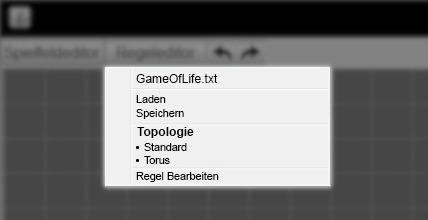
\includegraphics[width=15cm]{regeleditor_dropdown_edit} %   width = 5 für kleine Fenster, name == Name des Bildes ohne Dateiendung  

\begin{longtable}[m]{|m{2cm}|m{4cm}|m{9cm}|} % Die Tabelle für grobe Auflistung, mit dem Format
        \hline
        RF-01 & Laden & Ruft den Filechooser zum Laden eines anderen Regelausdrucks auf \\
        \hline
        RF-02 & Speichern & Ruft den Java-Swing-Filechooser zum Speichern des aktuellen Regelausdrucks auf. \\
        \hline
        RF-03 & Topologiewechsler & Auswahlschalter für das Spielfeldrandverhalten. \\
        \hline
        RF-04 & Regel Bearbeiten & Ruft das Popup-Fenster zum Regelausdruck bearbeiten auf. \\
        \hline
\end{longtable}
\pagebreak

    %Auflistung der einzelnen Funktionen: für jede davon eine Tabelle nach diesem Muster (Copy/paste sind am Start)

    \begin{tabular}[m]{|m{7cm}|m{9cm}|}
        \hline
        Anwendungsfall ID     & RF-01 \\ %Hier immer den rechten Tabelleneintrag ergänzen.
        \hline
        AF Name     &  Laden \\
        \hline
        Akteur&Benutzer des Programms \\
        \hline
        Vorbedingung&Programm gestartet, Benutzer lebendig, Regeleditor Dropdownmenü ausgewählt\\
        \hline
        Auslösendes Ereignis&Mausklick auf den Laden-Button\\
        \hline
        Nachbedingung Erfolg&Öffnen des Java-Swing-Fensters mit FileChooser zum öffnen einer Regeldatei\\
        \hline
        Nachbedingung Fehlschlag&Fehlermeldung und Rückkehr zur Haupt-Oberfläche.\\
        \hline
        Ablauf&Nutzer klickt auf Button und öffnet das Fenster zum laden einer Regeldatei. Durch auswählen und Bestätigen durch klick auf "Öffnen". wird die aktuell aktive Regel durch die geladene ersetzt.\\
        \hline
    \end{tabular}
    \par
    
    \begin{tabular}[m]{|m{7cm}|m{9cm}|}
        \hline
        Anwendungsfall ID     & RF-02 \\ %Hier immer den rechten Tabelleneintrag ergänzen.
        \hline
        AF Name     &  Speichern \\
        \hline
        Akteur&Benutzer des Programms \\
        \hline
        Vorbedingung&Programm gestartet, Benutzer lebendig, Regeleditor Dropdownmenü ausgewählt\\
        \hline
        Auslösendes Ereignis&Mausklick auf den Speichern-Button\\
        \hline
        Nachbedingung Erfolg&Öffnen des Java-Swing-Fensters mit FileChooser zum speichern einer Regeldatei\\
        \hline
        Nachbedingung Fehlschlag&Fehlermeldung und Rückkehr zur Haupt-Oberfläche.\\
        \hline
        Ablauf&Nutzer klickt auf Button und öffnet das Fenster zum Speichern einer Regeldatei. Durch auswählen und Bestätigen durch klick auf "Öffnen". wird die aktuell aktive Regel an besagter Stelle gespeichert.\\
        \hline
    \end{tabular}
    \par

    \begin{tabular}[m]{|m{7cm}|m{9cm}|}
        \hline
        Anwendungsfall ID     & RF-03 \\ %Hier immer den rechten Tabelleneintrag ergänzen.
        \hline
        AF Name     &  Topologie \\
        \hline
        Akteur&Benutzer des Programms \\
        \hline
        Vorbedingung&Programm gestartet, Benutzer lebendig, Regeleditor Dropdownmenü ausgewählt\\
        \hline
        Auslösendes Ereignis&Mausklick auf den Topologie-RadioButton\\
        \hline
        Nachbedingung Erfolg&Setzen der Spielfeldkantenbehandlung auf Torus oder Beschränkt, je nach Wunsch.\\
        \hline
        Nachbedingung Fehlschlag&Fehlermeldung und Rückkehr zur Haupt-Oberfläche.\\
        \hline
        Ablauf&Durch Klick auf "Standard" wird das Spielfeld als endliches Spielfeld behandelt, an den Kanten werden alle nachbarzellen als 0 angenommen.
        Durch klick auf "Torus" werden die Zellen an den Kanten die Zellen an gegenüberliegenden Kanten als Nachbarn behandeln.\\
        \hline
    \end{tabular}
    
    \pagebreak
    \par
    Regeleditor Popup-Fenster mit Texteingabe:
    \par
    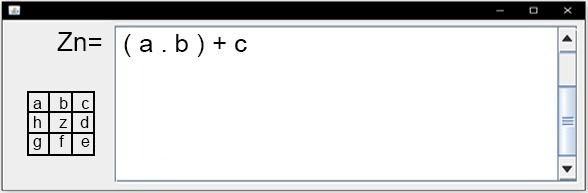
\includegraphics[width=15cm]{regedit}
    \par
    \begin{tabular}[m]{|m{5cm}|m{11cm}|}
        \hline
        Anwendungsfall ID     & RF-04 \\ %Hier immer den rechten Tabelleneintrag ergänzen.
        \hline
        AF Name     &  Regel Bearbeiten \\
        \hline
        Akteur&Benutzer des Programms \\
        \hline
        Vorbedingung&Programm gestartet, Benutzer lebendig, Dropdownmenü "Regeleditor" ausgewählt.\\
        \hline
        Auslösendes Ereignis&Mausklick auf den "Regel Bearbeiten"-Button im Regeleditor-Dropdownmenü\\
        \hline
        Nachbedingung Erfolg&Öffnen des Popupfensters "Regeleditor" (siehe oben).\\
        \hline
        Nachbedingung Fehlschlag&Fehlermeldung und Rückkehr zur Haupt-Oberfläche.\\
        \hline
        Ablauf&Öffnen des Übergangsregel-Editors. Bei Öffnen steht im Textfeld die zurzeit verwendete Transitionsregel. Durch Tastatureingabe kann der String im Textfeld verändert werden, womit die Transitionsregel angepasst wird. Ferner gibt es ein Bild links, welches als Hilfestellung die Variablen angibt, welche die Zellzustände von Nachbarzellen angeben. Auf die Weise kann der Zustand der akuell betrachteten Zelle für die nächste Iteration auf Basis ihrer Nachbarn berechnet werden\\
        \hline
    \end{tabular}
    \par
\subsubsection{}



\subsubsection{Datenverarbeitung}
\subsubsection{Datenspeicherung}
\subsection{Nichtfunktionale Anforderungen}
\subsubsection{Performance}
\begin{itemize}
    \item Lineare Laufzeit der Generationsberechnung pro Spielfeldgröße
\end{itemize}
\subsubsection{Zuverlässigkeit}
\begin{itemize}
    \item This is bleeding edge technology. Report bugs to Jehova's Witnesses, Ortsgruppe Westfalen-Lippe.
\end{itemize}

Hinweis: Für die Sicherheit des Nutzers wird nicht garantiert.
\pagebreak
\section{Testszenarien}
\subsection{UI}
Das UserInterface bietete einige Möglichkeiten für Probleme. Für alle Texteingabefelder muss zur Laufzeit geprüft werden, ob der User-Input in Ordnung ist und bei Bedarf Fehlermeldungen ausspucken. Beispiel: Die Spielfeldgröße muss unbedingt vom Typ int sein. "abeuiae" ist keine valide Spielfeldgröße.
Ferner muss geprüft werden, ob alle Knöpfe ausschließlich das tun, was sie sollen und nicht spaßige Nebeneffekte erzeugen.
\subsection{Verarbeitung}
Es muss geprüft werden, ob der Regelinterpreter vernünftig funktioniert. Es muss geprüft werden ob die Spielfeldvariation vernünftig funktioniert. Es muss geprüft werden ob die Arrayverarbeitung für den Spielstand venünftig funktioniert. 

\subsection{Speichern}
Der Java Filechooser wird wohl funktionieren, nicht wahr?

ggf. kann man einen Speicherzustand laden und unter anderem Namen speichern und dann den Inhalt vergleichen....
\subsection{Performance}
Awatt, Performance wird auf modernen Systemen in ausreichender Menge vorhanden sein. Bitte keine Speicherlecks bauen...
\subsection {Benutzbarkeit (Schimpanse benötigt)}
Bin kein Schimpanse, es 
\pagebreak
\section{Entwicklungsumgebung}
\subsection{Verwendete Software}
\begin{tabular}{|c|c|}
\hline
Betriebssysteme:     &  MacOS X, Windoof X, Linux X
  \\
     \hline
     Bildbearbeitung  \&  Diaagramme & 
         GIMP, Photoshop, Modelio
 \\
     \hline
     Programmierung  \& Versionierung & 
          Eclipse, 
          Eclipse Window builder,
          GIT\\
     \hline
\end{tabular}
\subsection{Verwendete Hardware}
Intelligente Frühstücksbrettchen mit abwaschbarer Benutzeroberfläche verschiedener Hubraumklassen.
\subsection{verwendete Organisation}
Haben Sie wirklich den Eindruck, dass hier irgendwas organisiert abläuft? 
Aber gut, ein Versuch: 
Wenn etwas schief geht, ist Alex schuld.
Wenn jemand Ahnung hat, dann Nico.
Wenn jemand Protokoll schreibt, dann Felix.
Wenn jemand gute Laune hat, dann Jörg.
Wenn jemand Photoshop macht, dann Diaa.

\pagebreak


\par
Glossar
\par
\begin{tabular}{|c|c|}
\hline
Begriff & Erklärung \\
    \hline
  Performance   & Geschwindigkeit der Software. \\
  \hline
JRE  & Java Runtime Environment. Ein Stück frei erhältliche Software, die es Ermöglicht Java Programme auszuführen. \\
    \hline
  & \\
    \hline
  & \\
    \hline
  & \\
    \hline
  & \\  
  \hline
  & \\
\end{tabular}


\end{document}
